%%%%%%%%%%%%%%%%%%%%%%%%%%%%%%%%%%%%%%%%%%%%%%%%%%%%%%%%%%%%%%%%%%%%%%%%%%%%%%%%%%%
%% This project aims to create the UFC template for presentation.                %%
%% author: Maurício Moreira Neto - Doctoral student in Computer Science (MDCC)   %%
%% contacts:                                                                     %%
%%    e-mail: maumneto@ufc.br                                                    %%
%%    linktree: https://linktr.ee/maumneto                                       %%
%%%%%%%%%%%%%%%%%%%%%%%%%%%%%%%%%%%%%%%%%%%%%%%%%%%%%%%%%%%%%%%%%%%%%%%%%%%%%%%%%%%
\documentclass{libs/ufc_format}
% Inserting the preamble file with the packages
%%%%%%%%%%%%%%%%%%%%%%%%%%%%%%%%%%%%%%%%%%%%%%%%%%%%%%%%%%%%%%%%%%%%%
%% This file contains the packages that can be used in the beamer. %%
%%%%%%%%%%%%%%%%%%%%%%%%%%%%%%%%%%%%%%%%%%%%%%%%%%%%%%%%%%%%%%%%%%%%%
% Package to fonts family
\usepackage[T1]{fontenc}
% Package to accentuation
\usepackage[utf8]{inputenc}
% Package to Portuguese language
\usepackage[brazil]{babel}
% Package to Figures
\usepackage{graphicx}
% Package to the colors
\usepackage{color}
% Package to the colors
\usepackage{xcolor}
% Packages to math symbols and expressions
\usepackage{amsfonts, amssymb, amsmath}
% Package to multiple lines and columns in table
\usepackage{multirow, array} 
% Package to create pseudo-code
% For more detail of this package: http://linorg.usp.br/CTAN/macros/latex/contrib/algorithm2e/doc/algorithm2e.pdf
\usepackage{algorithm2e}
% Package to insert code
\usepackage{listings} 
\usepackage{keyval}
% Package to justify text
\usepackage[document]{ragged2e}
% Package to manage the bibliography
\usepackage[backend=biber, style=numeric, sorting=none]{biblatex}
% Package to facilities quotations
\usepackage{csquotes}
% Package to use multicols
\usepackage{multicol}

% Packages added by me
\usepackage{url}
\usepackage{tikz}
%\usepackage{multimedia}
%\usepackage{media9}[playbutton=plain, windowed=1280x720]
% Inserting the references file
\bibliography{references.bib}
\renewcommand*{\bibfont}{\scriptsize}

% Title
\title[Introdução a IA]{\huge\textbf{Introdução à Inteligência Artificial}}
% Subtitle
%\subtitle{Parte 3}
% Author of the presentation
\author{Evandro J.R. Silva}
% Institute's Name
\institute[Estácio Teresina]{
    % email for contact
    \normalsize{\email{ejrs.profissional@gmail.com}}
    \newline
    % Department Name
    %\department{Bacharelado em Ciência da Computação}
    \newline
    % university name
    %\ufc
    \estaciothe
}
% date of the presentation
\date{30 e 31 de Janeiro}


%%%%%%%%%%%%%%%%%%%%%%%%%%%%%%%%%%%%%%%%%%%%%%%%%%%%%%%%%%%%%%%%%%%%%%%%%%%%%%%%%%
%% Start Document of the Presentation                                           %%               
%%%%%%%%%%%%%%%%%%%%%%%%%%%%%%%%%%%%%%%%%%%%%%%%%%%%%%%%%%%%%%%%%%%%%%%%%%%%%%%%%%
\begin{document}
% insert the code style
%%%%%%%%%%%%%%%%%%%%%%%%%%%%%%%%%%%%%%%%%%%%%%%%%%%%%%%%%%%%%%%%%%%%%%%%%%%%%%%%%%%
%% This file contains the style of the codes show in slides.                     %%
%% The package used is listings, but it possible to used others.                 %%
%%%%%%%%%%%%%%%%%%%%%%%%%%%%%%%%%%%%%%%%%%%%%%%%%%%%%%%%%%%%%%%%%%%%%%%%%%%%%%%%%%%

% color used in the code style
\definecolor{codegreen}{rgb}{0,0.6,0}
\definecolor{codegray}{rgb}{0.5,0.5,0.5}
\definecolor{codepurple}{rgb}{0.58,0,0.82}
\definecolor{codebackground}{rgb}{0.95,0.95,0.92}

% style of the code!
\lstdefinestyle{codestyle}{
    backgroundcolor=\color{codebackground},   
    commentstyle=\color{codegreen},
    keywordstyle=\color{magenta},
    numberstyle=\tiny\color{codegray},
    stringstyle=\color{codepurple},
    basicstyle=\ttfamily\footnotesize,
    frame=single,
    breakatwhitespace=false,         
    breaklines=true,                 
    captionpos=b,                    
    keepspaces=true,                 
    numbers=left,                    
    numbersep=5pt,                  
    showspaces=false,                
    showstringspaces=false,
    showtabs=false,                  
    tabsize=2,
    title=\lstname 
}

\lstset{style=codestyle}


%% ---------------------------------------------------------------------------
% First frame (with tile, subtitle, ...)
\begin{frame}{}
    \maketitle
\end{frame}

%% ---------------------------------------------------------------------------
% Second frame
\begin{frame}{Sumário}
    \begin{multicols}{2}
        \tableofcontents
    \end{multicols}
\end{frame}

%=============================================================================
% SECTION 1
%=============================================================================
\section{O que é IA?}

\begin{frame}{}
    \centering
    \Large
    O que é Inteligência Artificial?
\end{frame}

\begin{frame}{O que é IA}
    \begin{itemize}
        \justifying
        \item Como definir a inteligência?
        \item<2-> Como definir uma inteligência artificial?\\
        \uncover<3>{
        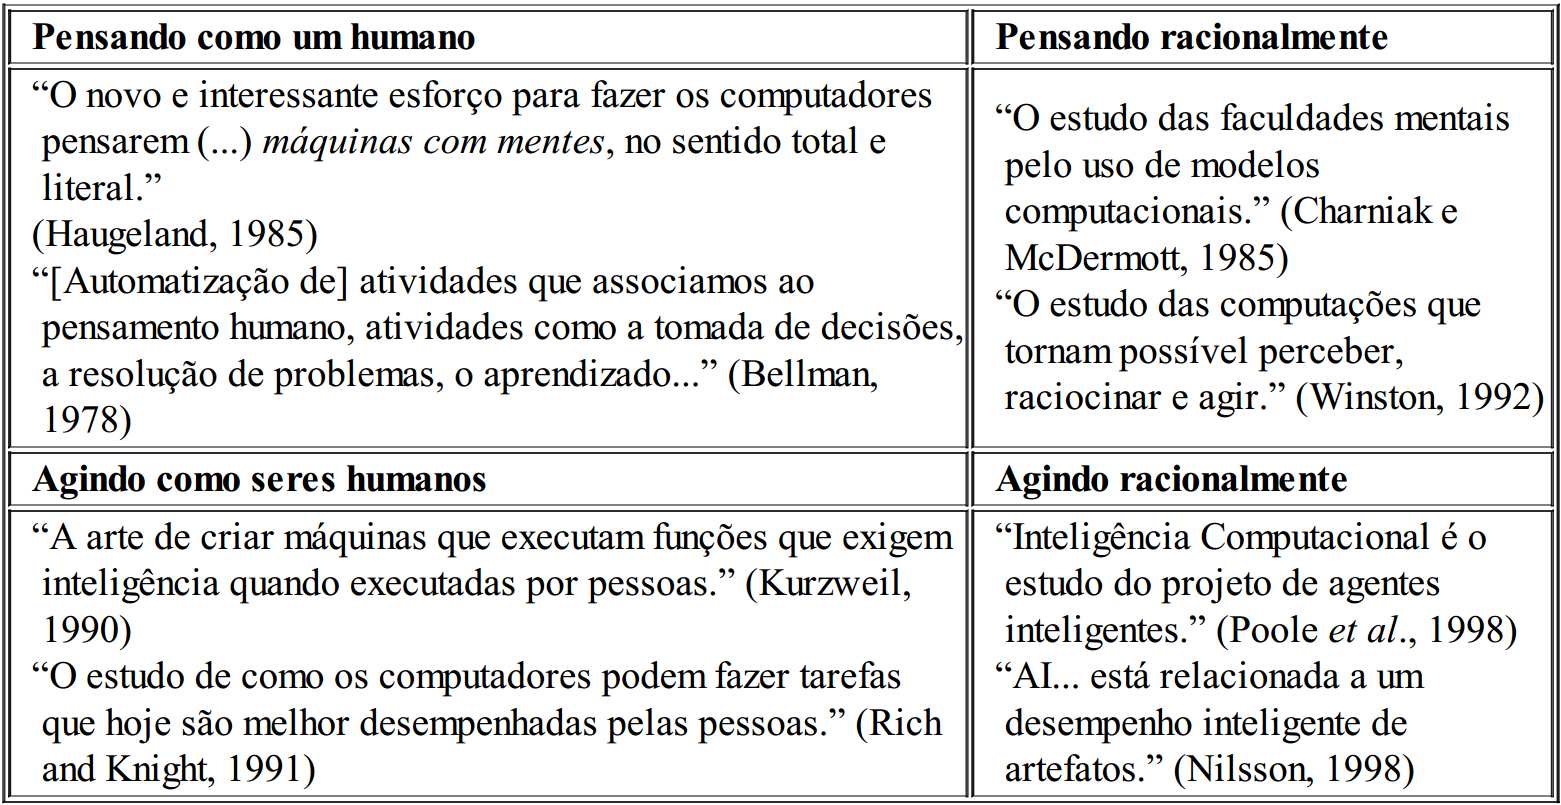
\includegraphics[width=0.9\textwidth]{figuras/figura01.png}
        }
    \end{itemize}
\end{frame}

%-----------------------------------------------------------------------------
% SUBSECTION 1.1
%-----------------------------------------------------------------------------
\subsection{Fundamentos da IA}

\begin{frame}{Fundamentos da IA}
    \begin{itemize}
        \justifying
        \item Breve fundamentação da Inteligência artificial:
            \begin{itemize}
                \item<2> Filosofia;
                \item<2> Matemática;
                \item<2> Economia;
                \item<2> Neurociência;
                \item<2> Psicologia;
                \item<2> Engenharia de computadores;
                \item<2> Teoria de controle e cibernética;
                \item<2> Linguística.
            \end{itemize}
    \end{itemize}
\end{frame}

\begin{frame}{Fundamentos da IA}
    \begin{itemize}
        \justifying
        \item Filosofia
            \begin{itemize}
                \justifying
                \item<1> Regras formais podem ser usadas para obter conclusões válidas?
                \item<1> Como a mente (o intelecto) se desenvolve a partir de um cérebro físico?
                \item<1> De onde vem o conhecimento?
                \item<1> Como o conhecimento conduz à ação?
            \end{itemize}
        \item<2-> Matemática
            \begin{itemize}
                \justifying
                \item<2> Quais são as regras formais para obter conclusões válidas?
                \item<2> O que pode ser computado?
                \item<2> Como raciocinamos informações incertas?
            \end{itemize}
    \end{itemize}
\end{frame}

\begin{frame}{Fundamentos da IA}
    \begin{itemize}
        \justifying
        \item Economia
            \begin{itemize}
                \justifying
                \item<1> Como devemos tomar decisões para maximizar a recompensa?
                \item<1> Como devemos fazer isso quando outros não podem nos acompanhar?
                \item<1> Como devemos fazer isso quando a recompensa pode estar distante no futuro?
            \end{itemize}
        \item<2-> Neurociência
            \begin{itemize}
                \justifying
                \item<2> Como o cérebro processa informações?
            \end{itemize}
        \item<3-> Psicologia
            \begin{itemize}
                \justifying
                \item<3> Como os seres humanos e os animais pensam e agem?
            \end{itemize}
        \item<4-> Engenharia de computadores
            \begin{itemize}
                \justifying
                \item<4> Como podemos construir um computador eficiente?
            \end{itemize}
    \end{itemize}
\end{frame}

\begin{frame}{Fundamentos da IA}
    \begin{itemize}
        \justifying
        \item Teoria de controle e cibernética
            \begin{itemize}
                \justifying
                \item<1> Como os artefatos podem operar sob seu próprio controle?
            \end{itemize}
        \item<2-> Linguística
            \begin{itemize}
                \justifying
                \item<2> Como a linguagem se relaciona com o pensamento?
            \end{itemize}
    \end{itemize}
\end{frame}

%=============================================================================
% SECTION 2
%=============================================================================
\section{História da IA}

\begin{frame}{}
    \centering
    \Large
    História da IA
\end{frame}

%-----------------------------------------------------------------------------
% SUBSECTION 2.1
%-----------------------------------------------------------------------------
\subsection{``Gestação''}

\begin{frame}{``Gestação''}
    \begin{itemize}
        \justifying
        \item \textbf{1943}: Warren McCulloch e Walter Pitts propuseram um modelo de neurônios artificiais, no qual cada neurônio se caracteriza por estar ``ligado'' ou ``desligado''. O estado \alert{ligado} é análogo a um neurônio estimulado.\\
        \uncover<2>{
            \centering
            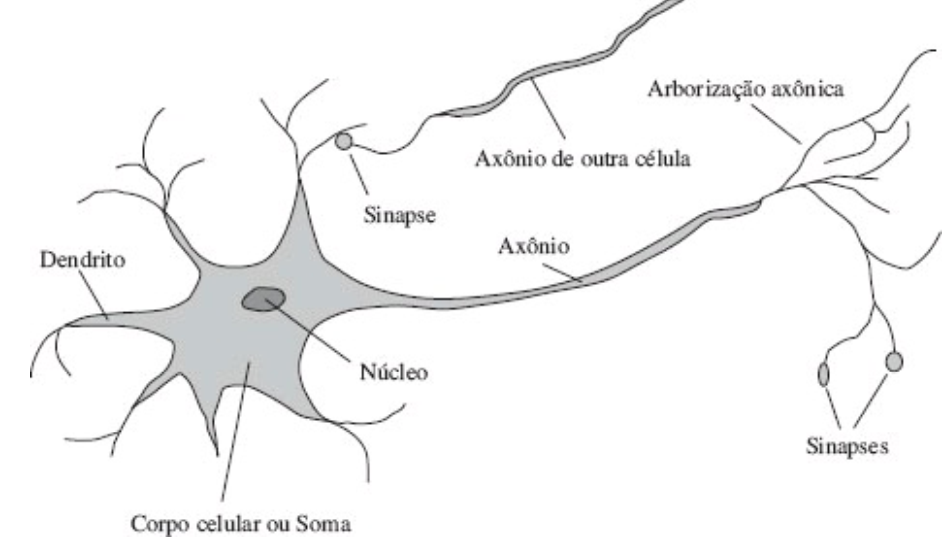
\includegraphics[width=0.85\textwidth]{figuras/figura02.png}
            }
    \end{itemize}
\end{frame}

\begin{frame}{``Gestação''}
    \begin{itemize}
        \justifying
        \item<1> \textbf{1949}: Donald Hebb demonstrou uma regra de atualização simples para modificar as intensidades de conexão entre neurônios. Ficou conhecido como \textbf{aprendizagem hebbiana}: ``o peso sináptico entre dois neurônios aumenta se ambos são ativados simultaneamente, e reduz se são ativados separadamente''.
        \item<2-> \textbf{1950}: 
            \begin{itemize}
                \justifying
                \item<2> Marvin Minsky e Dean Edmonds, alunos de Harvard, constroem o SNARC, o primeiro computador de rede neural, o qual usada 3000 válvulas eletrônicas e um mecanismo de piloto automático retirado de um bombardeiro B-24.
                \item<3> Alan Turing publica \textit{Computing Machinery and Intelligence}, onde apresenta o famoso \textbf{teste de Turing}, algoritmos genéticos e aprendizagem por reforço.
            \end{itemize}
    \end{itemize}
\end{frame}

%-----------------------------------------------------------------------------
% SUBSECTION 2.2
%-----------------------------------------------------------------------------
\subsection{``Nascimento''}

\begin{frame}{``Nascimento''}
    \begin{itemize}
        \justifying
        \item \textbf{1956}: 
            \begin{itemize}
                \justifying
                \item<1> John McCarthy, Minsky, Claude Shannon e Nathaniel Rochester organizaram um seminário de dois meses em Dartmouth College. A proposta: ``[...] um estudo de dois meses e dez homens sobre inteligência artificial [...] para prosseguir com a conjectura básica de que cada aspecto da aprendizagem ou qualquer outra característica da inteligência pode, em princípio, ser descrita tão precisamente a ponto de ser construída uma máquina para simulá-la''.
                \item<2> Allen Newell e Hebert Simon, da Carnegie Tech, apresentaram o programa \textit{Logic Theorist}, o qual foi capaz de demonstrar a maioria dos teoremas do capítulo 2 do livro \textit{Principia Mathematica} escrita por Russel e Whitehead. O programa havia sido capaz de criar uma prova de um teorema mais curta que a do livro.
            \end{itemize}
    \end{itemize}
\end{frame}

%-----------------------------------------------------------------------------
% SUBSECTION 2.3
%-----------------------------------------------------------------------------
\subsection{``Crescimento'' e grandes expectativas}

\begin{frame}{``Crescimento'' e grandes expectativas}
    \begin{itemize}
        \justifying
        \small
        \item<1-2> É interessante lembrar que os computadores ainda eram relativamente primitivos, e alguns anos antes eram vistos como objetos capazes de efetuar operações aritméticas e nada mais.
        \item<2-3> Newel e Simon prosseguiram do \textit{Logistic Theorist} para o \textit{General Problem Solver};
        \item<3-4> Herbert Gelernter (1959) construiu o \textit{Geometry Theorem Prover}, que podia demonstrar teoremas que seriam considerados bastante complicados por muitos alunos de matemática.
        \item<4-5> Desde 1952 Arthur Samuel escreveu uma série de programas para jogos de damas que eventualmente aprendiam a jogar em um nível amador elevado. Seu programa, que já jogava melhor do que ele, foi apresentado na televisão em fevereiro de 1956.
        \item<5-6> John McCarthy saiu de Dartmouth para o MIT e, em 1958, definiu a linguagem de programação \textbf{Lisp}.
        \item<6> As redes neurais, iniciadas por McCulloch e Pitts, receberam contribuições de Winograd e Cowan (1963), e o aprendizado Hebbiano foi aperfeiçoado por Bernie Widrow (1960 e 1962, com suas redes adalines) e Frank Rosenblatt (1962, com os perceptrons).
    \end{itemize}
\end{frame}

%-----------------------------------------------------------------------------
% SUBSECTION 2.4
%-----------------------------------------------------------------------------
\subsection{Dose de realidade}

\begin{frame}{Dose de realidade (1966 - 1973)}
    \begin{itemize}
        \justifying
        \item Os pesquisadores de IA eram ousados nos prognósticos de seus sucessos futuros.\\
            \begin{block}{Declaração de Hebert Simon (1957)}
                \justifying
                Não é meu objetivo surpreendê-los ou chocá-los, mas o modo mais simples de resumir tudo isso é dizer que agora existem no mundo máquinas que pensam, aprendem e criam. Além disso, sua capacidade de realizar essas atividades está crescendo rapidamente até o ponto --- em um futuro visível --- no qual a variedade de problemas com que elas poderão lidar será correspondente à variedade de problemas com os quais lida a mente humana.
            \end{block}
        \end{itemize}
\end{frame}

\begin{frame}{Dose de realidade (1966 - 1973)}
    \begin{itemize}
        \justifying
        \item<1-2> Simon fez outras predições mais concretas: dentro de 10 anos um computador seria camperão de xaderz e um teorema matemático significativo seria provado por uma máquina.
        \item<2> O que ele predisse aconteceu de fato, mas só uns 40 anos depois.
        \item<3-> O desempenho dos algoritmos era promissor, mas os testes foram feitos em exemplos simples.
        \item<4-> Tais algoritmos falharam desastrosamente quando lidaram com conjuntos de problemas mais extensos ou mais difíceis.
        \item<5-> Um dos exemplos icônicos: a tradução do Russo para o Inglês. A tradução é muito mais complexa do que substituir cada palavra pelo seu equivalente em um dicionário.
    \end{itemize}
\end{frame}

\begin{frame}{Dose de realidade (1966 - 1973)}
    \begin{itemize}
        \justifying
        \item Vários relatórios governamentais foram apontando não somente as falhas mas também as graves limitações da IA.\\
        \centering
        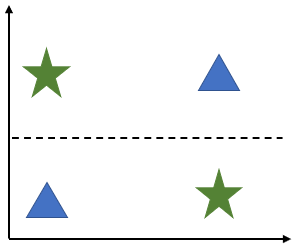
\includegraphics[width=0.2\textwidth]{figuras/perceptron_1}
        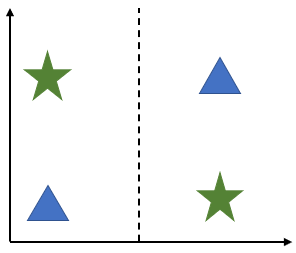
\includegraphics[width=0.2\textwidth]{figuras/perceptron_2}\\
        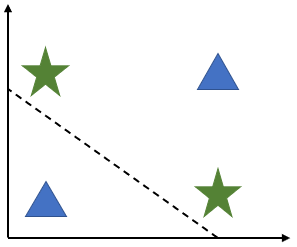
\includegraphics[width=0.2\textwidth]{figuras/perceptron_3}
        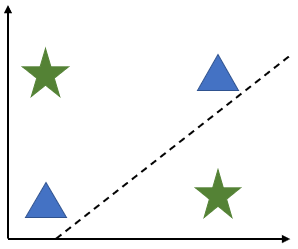
\includegraphics[width=0.2\textwidth]{figuras/perceptron_4}\\
        \justifying
        \item Esperava-se que melhorias de hardware subsequentes fossem resolver logo os problemas, porém a ``explosão combinatória'' para a resolução dos problemas mostrou que a melhoria do hardware não era viável.
        \item<2> Os governos foram então encerrando seus apoios a pesquisa em IA.
    \end{itemize}
\end{frame}

%-----------------------------------------------------------------------------
% SUBSECTION 2.5
%-----------------------------------------------------------------------------
\subsection{Sistemas baseados em conhecimento}

\begin{frame}{Sistemas baseados em conhecimento (1969 - 1979)}
    \begin{itemize}
        \justifying
        \item<1> De início os pesquisadores de IA procuravam um mecanismo de uso geral para reunir passos elementares de raciocínio para encontrar soluções completas.
        \item<1> Tais abordagens foram chamadas \textbf{métodos fracos} porque, embora gerais, não podiam ter aumento de escala para instâncias de problemas grandes ou difíceis.
        \item<2> Alternativa: usar um conhecimento mais amplo e específico de domínio que permita passos de raciocínio maiores e que possam tratar com mais facilidade casos que ocorrem tipicamente em especialidades estritas.
    \end{itemize}
\end{frame}

\begin{frame}{Sistemas baseados em conhecimento (1969 - 1979)}
    \begin{itemize}
        \justifying
        \item \textbf{DENDRAL} (1969)
            \begin{itemize}
                \justifying
                \item Desenvolvido em Stanford por Ed Feigenbaum (antigo aluno de Simon), Bruce Buchanan (filósofo transformado em cientista da computação) e Joshua Lederberg (geneticista laureado com um Nobel).
                \item<2> Objetivo: resolver o problema de inferir a estrutura molecular a partir das informações fornecidas por um espectrômetro de massa.
                \item<2> A entrada para o programa consiste na fórmula elementar da molécula (por exemplo, $C_{6}H_{13}NO_{2}$) e o espectro de massa que fornece as massas dos diversos fragmentos da molécula gerada quando ela é bombardeada por um feixe de elétrons.
                \item<2> Por exemplo, o espectro de massa poderia conter um pico em m = 15, correspondendo à massa de um fragmento metil ($CH_{3}$).
            \end{itemize}
    \end{itemize}
\end{frame}

\begin{frame}{Sistemas baseados em conhecimento (1969 - 1979)}
    \begin{itemize}
        \justifying
        \item \textbf{DENDRAL} (1969)
            \begin{itemize}
                \justifying
                \item A versão ingênua do programa gerou todas as estruturas possíveis consistentes com a fórmula e depois previu qual seria o espectro de massa observado para cada uma, comparando esse espectro com o espectro real.
                \item<2> Sua importância vem do fato de ter sido o primeiro sistema bem-sucedido de \textit{conhecimento intensivo}, ou seja, solucionou um problema tendo por base o conhecimento de especialistas.
            \end{itemize}
    \end{itemize}
\end{frame}

\begin{frame}{Sistemas baseados em conhecimento (1969 - 1979)}
    \begin{itemize}
        \justifying
        \item Após o DENDRAL, outros sistemas especialistas, em diversas áreas, incluindo Processamento de Linguagem Natural foram surgindo e sendo bem sucedidos.
        \item<2-> A IA passou a ser uma nova ``indústria'', com a produção de sistemas comerciais
            \begin{itemize}
                \justifying
                \item<3-4> R1, o primeiro sistema especialista comercial bem sucedido, ajudava a configurar pedidos de novos sistemas de computadores. Em 1986 fez com que a empresa \textit{Digital Equipment Corporation} economizasse cerca de 40 milhões de dólares.
                \item<4> Em 1988 a empresa Du Pont tinha 100 sistemas especialistas em uso e 500 em desenvolvimento, economizando aproximadamente 10 milhões de dólares por ano.
            \end{itemize}
        \item<5> Alguns fundos de pesquisa governamentais que haviam sido suspendidos, voltaram. Mas ainda assim, os projetos nunca alcançaram seus objetivos ambiciosos.
    \end{itemize}
\end{frame}

%-----------------------------------------------------------------------------
% SUBSECTION 2.6
%-----------------------------------------------------------------------------
\subsection{O retorno das Redes Neurais}

\begin{frame}{O retorno das Redes Neurais (1986)}
    \begin{itemize}
        \justifying
        \item Um algoritmo de aprendizado, chamado de \textbf{retropropagação} (mais conhecido com seu termo em Inglês \textit{backpropagation}), que havia sido inventado em 1969 por Bryson e Ho, foi reinventado na década de 80.
        \item<2> O algoritmo foi aplicado a muitos problemas de aprendizado em ciência da computação e psicologia, e seus resultados foram disseminados na coletânea \textit{Parallel Distributed Processing} (Rumelhart e McClelland, 1986).
    \end{itemize}
\end{frame}

%-----------------------------------------------------------------------------
% SUBSECTION 2.7
%-----------------------------------------------------------------------------
\subsection{A IA se torna uma ciência}

\begin{frame}{A IA se torna uma ciência (1987)}
    \begin{itemize}
        \justifying
        \item O método científico foi adotado com firmeza.
        \item Para serem aceitas, as hipóteses devem ser submetidas a rigorosos experimentos empíricos, e os resultados devem ser analisados estatisticamente de acordo com sua importância.
        \item Experimentos agora podem ser replicados a partir da utilização de repositórios compartilhados de código e dados.
    \end{itemize}
\end{frame}

%-----------------------------------------------------------------------------
% SUBSECTION 2.8
%-----------------------------------------------------------------------------
\subsection{O surgimento de Agentes Inteligentes}

\begin{frame}{O surgimento de Agentes Inteligentes (1995)}
    \begin{itemize}
        \justifying
        \item O progresso da resolução de subproblemas da IA encorajou o retorno da pesquisa de ``um agente como um todo''.
        \item A Internet se tornou um dos ambientes mais importantes para os agentes inteligentes
            \begin{itemize}
                \justifying
                \item<2> Bots;
                \item<2> Sistemas de recomendação;
            \end{itemize}
        \item<3-> ``Pequeno problema'': subcampos isolados precisam ser reorganizados para a abordagem do problema maior
            \begin{itemize}
                \justifying
                \item<4> Sistemas sensoriais podem não fornecer informações perfeitamente confiáveis sobre um determinado ambiente. Portanto, é necessário acoplar sistemas de raciocínio e planejamento para lidar com as incertezas.
            \end{itemize}
    \end{itemize}
\end{frame}

%-----------------------------------------------------------------------------
% SUBSECTION 2.9
%-----------------------------------------------------------------------------
\subsection{Disponibilidade de conjuntos de dados muito grandes}

\begin{frame}{Disponibilidade de conjuntos de dados muito grandes (2001)}
    \begin{itemize}
        \justifying
        \item Com o \textit{boom} da Internet, cada vez mais dados começaram a ser produzidos.
        \item Por volta de 2005 já tínhamos as primeiras redes sociais (praticamente programas de chat), e compartilhávamos gifs, fotos e vídeos (curtos e de baixa qualidade).
        \item Ao fim da década tínhamos redes sociais com centenas de milhões a até 1 bilhão de usuários, todos gerando e compartilhando muitos dados.
    \end{itemize}
\end{frame}

\begin{frame}{Disponibilidade de conjuntos de dados muito grandes (2001)}
    \centering
    
\includegraphics[width=0.45\textwidth]{figuras/msn_logo}
    
\includegraphics[width=0.45\textwidth]{figuras/kazaa_logo}\\
    
\includegraphics[width=0.4\textwidth]{figuras/mirc_logo}
    
\includegraphics[width=0.4\textwidth]{figuras/orkut_logo}
\end{frame}

\begin{frame}{Disponibilidade de conjuntos de dados muito grandes (2001)}
    \centering
    
\includegraphics[width=0.35\textwidth]{figuras/twitter_logo}
    
\includegraphics[width=0.35\textwidth]{figuras/facebook_logo}\\
    
\includegraphics[width=0.45\textwidth]{figuras/flogao_logo}
\end{frame}

%-----------------------------------------------------------------------------
% SUBSECTION 2.10
%-----------------------------------------------------------------------------
\subsection{O Estado da Arte}

\begin{frame}{O Estado da Arte (2011 - ?)}
    \centering
    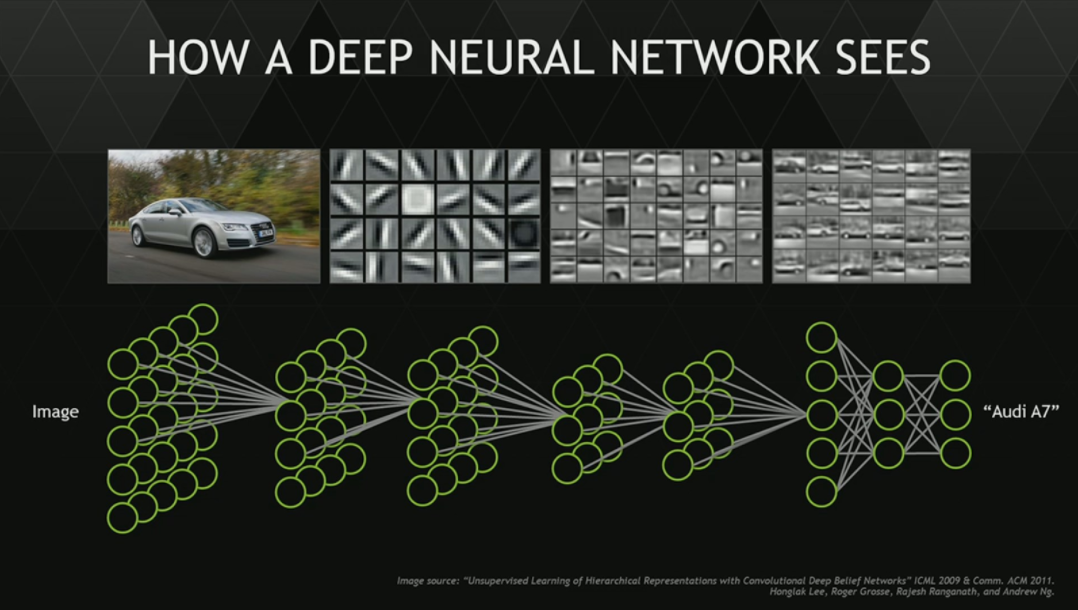
\includegraphics[width=\textwidth]{figuras/deeplearning}
\end{frame}

\begin{frame}{O Estado da Arte (2011 - ?)}
    \centering
    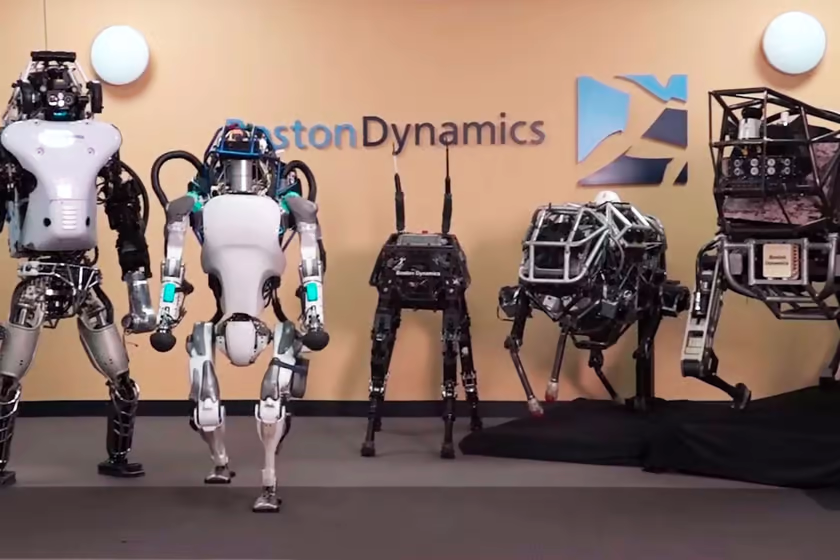
\includegraphics[width=0.9\textwidth]{figuras/boston_dynamics}
\end{frame}

\begin{frame}{O Estado da Arte (2011 - ?)}
    \begin{itemize}
        \item \href{https://openai.com/}{\underline{OpenAI}}
            \begin{itemize}
                \item \href{https://openai.com/blog/chatgpt/}{\underline{ChatGPT}}
                \item \href{https://openai.com/dall-e-2/}{\underline{DALL$\cdot$E}}
            \end{itemize}
    \end{itemize}
    \centering
    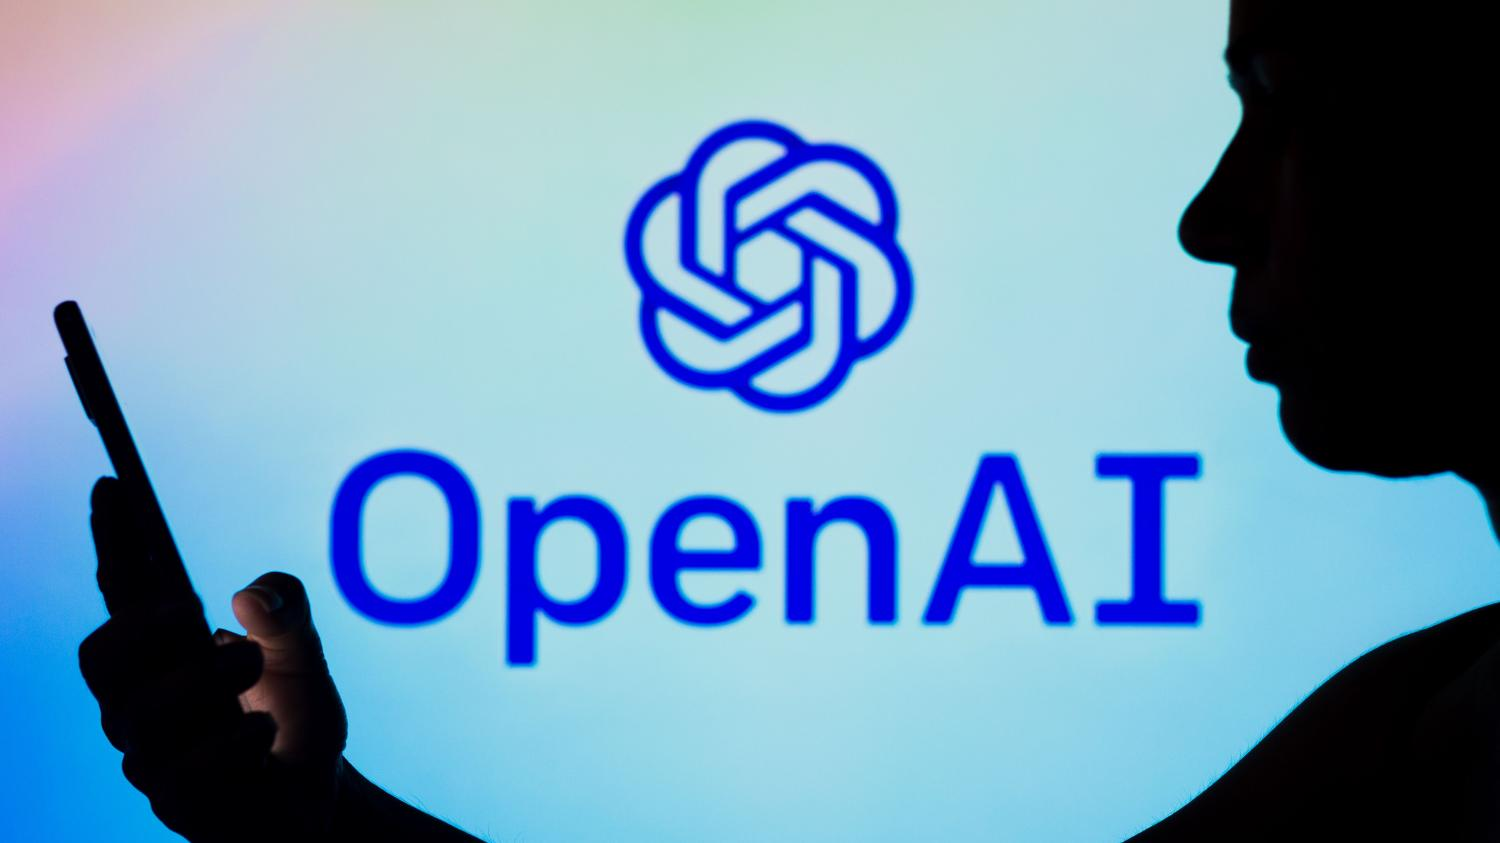
\includegraphics[width=0.75\textwidth]{figuras/openai}
\end{frame}

\begin{frame}{O Estado da Arte (2011 - ?)}
    \centering
    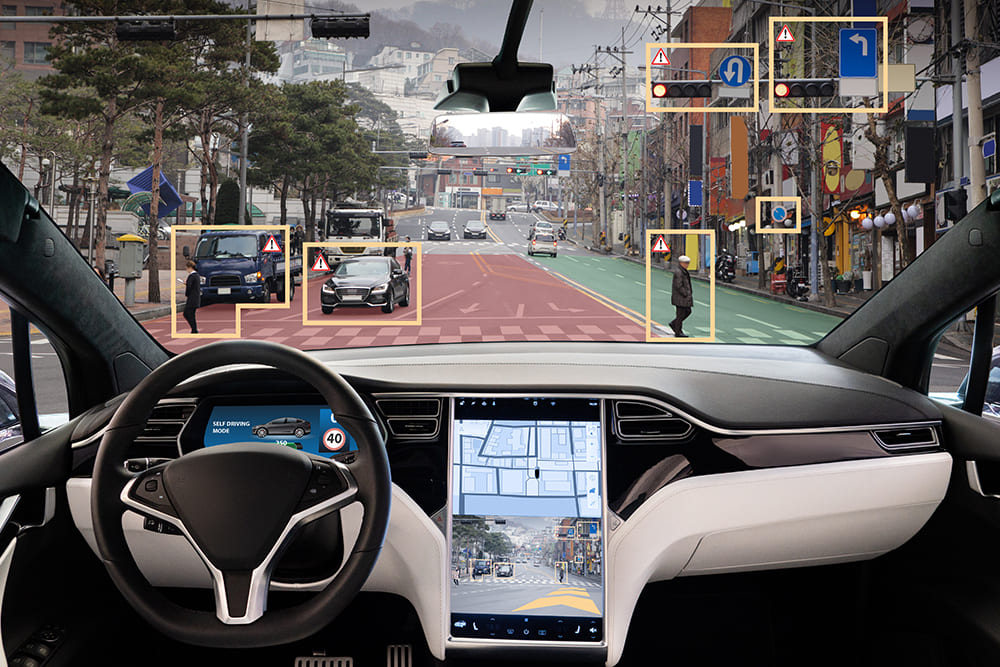
\includegraphics[width=\textwidth]{figuras/tesla}
\end{frame}

\begin{frame}{O Estado da Arte (2011 - ?)}
    \centering
    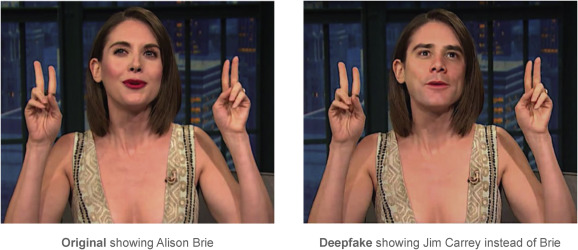
\includegraphics[width=\textwidth]{figuras/deepfake}
\end{frame}

%=============================================================================
% SECTION ?
%=============================================================================
\section{FIM}

\begin{frame}{}
    \centering
    \Large
    Terminamos a Primeira Parte!\\
    Obrigado pela atenção!
\end{frame}

%=============================================================================
% SECTION REFERENCES
%=============================================================================
%\begin{frame}[allowframebreaks]{Referências}
%    \scriptsize
%    \printbibliography
%\end{frame}

\end{document}













%% ---------------------------------------------------------------------------
% This presentation is separated by sections and subsections
%\section{Seção I}
%\begin{frame}{Explicações}
%    % itemize
%    Este é um template que pode ser utilizado para:
%    \begin{itemize}
%        \item Apresentação de Trabalhos Acadêmicos
%        \item Apresentação de Disciplinas
%        \item Apresentações de Teses e Dissertações
%    \end{itemize}
%
%    \vspace{0.4cm} % vertical space
%    
%    % enumeration
%    Para utilizar este template corretamente é importante que:
%    \begin{enumerate}
%        \item Tenha conhecimento mínimo sobre LaTeX
%        \item Ler os comentários no template (explicações)
%        \item Ler o README.md (documentação)
%    \end{enumerate}
%
%    \vspace{0.2cm}

%    \example{Este é um texto de exemplo!} \emph{Texto de Ênfase!}
%\end{frame}

%% ---------------------------------------------------------------------------
%\subsection{Subseção I}
%\begin{frame}{Criando Blocos}
%    % Blocks styles
%    \begin{block}{Bloco Padrão}
%        Texto do corpo do bloco.
%    \end{block}

%    \begin{alertblock}{Bloco de Alerta}
%        Texto do corpo do bloco.
%    \end{alertblock}
%
%    \begin{exampleblock}{Bloco de Exemplo}
%        Texto do corpo do bloco.
%    \end{exampleblock}   
%\end{frame}

%% ---------------------------------------------------------------------------
%\subsection{Subseção II}
%\begin{frame}{Criando Caixas}
%    \successbox{testando o success box}
%
%    \pause
%
%    \alertbox{testando o alert box}
%
%    \pause
%
%    \simplebox{testando o simple box}
%\end{frame}

%% ---------------------------------------------------------------------------
%\subsection{Subseção III}
%\begin{frame}{Criando Algoritmos (Pseudocódigo)}
%    \begin{algorithm}[H]
%        \SetAlgoLined
%        \LinesNumbered
%        \SetKwInOut{Input}{input}
%        \SetKwInOut{Output}{output}
%        \Input{x: float, y: float}
%        \Output{r: float}
%        \While{True}{
%          r = x + y\;
%          \eIf{r >= 30}{
%           ``O valor de $r$ é maior ou iqual a 10.''\;
%           break\;
%           }{
%           ``O valor de $r$ = '', r\;
%          }
%         } 
%         \caption{Algorithm Example}
%    \end{algorithm}
%\end{frame}

%% ---------------------------------------------------------------------------

%\begin{frame}{Inserindo Algoritmos}
%    \lstset{language=Python}
%    \lstinputlisting[language=Python]{code/main.py}
%\end{frame}

%% ---------------------------------------------------------------------------
%\begin{frame}{Inserindo Algoritmos}
%    \lstinputlisting[language=C]{code/source.c}
%\end{frame}

%% ---------------------------------------------------------------------------
%\begin{frame}{Inserindo Algoritmos}
%    \lstinputlisting[language=Java]{code/helloworld.java}
%\end{frame}

%% ---------------------------------------------------------------------------
%\begin{frame}{Inserindo Algoritmos}
%    \lstinputlisting[language=HTML]{code/index.html}
%\end{frame}

%% ---------------------------------------------------------------------------
% This frame show an example to insert multicolumns
%\section{Multicolunas}
%\begin{frame}{Seção II - Multicolunas}
%    \begin{columns}{}
%        \begin{column}{0.5\textwidth}
%            \justify
%            É possível colocar mais de uma coluna utilizando os comandos de $\backslash$begin\{column\}\{\} e $\backslash$end\{column\}
%        \end{column}
%        \begin{column}{0.5\textwidth}
%            \justify
%            Porém, o espaçamento deve ser proporcional entre as colunas para que estas colunas não entrem em coflito. O espaçamento é dado pelo segundo argumento do $\backslash$begin.
%        \end{column}
%    \end{columns}    
%\end{frame}

%% ---------------------------------------------------------------------------
% This frame show an example to insert figures
%\section{Imagens}
%\begin{frame}{Seção III - Figures}
%    \begin{figure}
%        \centering
%        \caption{Emblema da UFC.}
%        
\includegraphics[scale=0.3]{libs/emblemufc.pdf}
%        \source{Obtido pelo site oficial da UFC \cite{siteufc} \cite{einstein}}
%        \label{fig:ufc_emblem}
%    \end{figure}
%\end{frame}

%% ---------------------------------------------------------------------------
% Reference frames
%\begin{frame}[allowframebreaks]
%    \frametitle{Referências}
%    \printbibliography
%\end{frame}

%% ---------------------------------------------------------------------------
% Final frame
%\begin{frame}{}
%    \centering
%    \huge{\textbf{\example{Obrigado(a) pela Atenção!}}}
%    
%    \vspace{1cm}
%    
%    \Large{\textbf{Contato:}}
%    \newline
%    \vspace*{0.5cm}
%    \large{\email{usuario@dominio}}
%\end{frame}